\documentclass[12pt,a4paper]{article}
\usepackage{preamble} % preamble.sty
% -----------------------------------------------------------------


\begin{document}
% Титульная страница (файл title.tex)
\begin{titlepage}
	\centering
	
	{\Large Санкт-Петербургский Государственный Университет \par}
	
	\vspace{0.5cm}
	
	{\large Факультет математики и механики\par}
	
	\vspace{7.5cm}
	
	{\Huge\bfseries Теория вероятностей} % Название

        \vspace{0.3cm}
	
        {\large Лектор: Зайцев~А.~Ю.}
        
        \vspace{1cm}
        
        {\Large 5 семестр}


\end{titlepage}
% Содержание
\tableofcontents
\newpage
% - - - - - - - - - - - - - - - - - -

\section{Лекция 02.09.25}
В средние века довольно популярной была игра в кости. На гранях кубика изображены числа из множества $\{1, 2, 3, 4, 5, 6\}$. Если предположить, что кубик идеален (т.е. симметричен и однороден), и подбрасывается в идеальных условиях без посторонних воздействий, то у нас нет объективных причин считать одну грань более предпочтительной, чем другую. Такие элементарные исходы являются равновозможными.

В таком случае, вероятность выпадения любой конкретной грани, например, шестёрки, определяется как отношение числа благоприятствующих исходов к общему числу всех возможных равновероятных исходов: $\mathbb{P}(\text{``выпала шестёрка''}) = \frac{1}{6}.$

Аналогично, вероятность события ``выпало чётное число'' (исходы: $2, 4, 6$) будет равна: $\mathbb{P}(\text{``чётное число''}) = \frac{3}{6} = \frac{1}{2}.$

Это классическое определение вероятности, которое эффективно, когда пространство исходов конечно и исходы равновозможны. Однако для более сложных задач (бесконечные пространства, неравновозможные исходы) потребуется более общий аксиоматический подход.

\begin{remind}
Комбинаторика предоставляет инструменты для подсчёта числа исходов, что часто помогает в вычислении вероятностей по классическому определению:
\begin{itemize}
    \item Число перестановок из $n$ различных элементов: $$n!$$
    \item Размещения: Число способов выбрать $k$ элементов из $n$ (порядок важен): $$A_n^k = \frac{n!}{(n-k)!}$$
    \item Сочетания: Число способов выбрать $k$ элементов из $n$ (порядок не важен): $$C_n^k = \binom{n}{k} = \frac{n!}{k! \cdot (n-k)!}$$
\end{itemize}
\end{remind}

\begin{definition}[Колмогоровская модель]
    \textit{Вероятностное пространство} -- тройка $\left( \Omega, \mathcal{F}, \mathbb{P} \right)$, где \begin{itemize}
        \item $\Omega$ -- множество элементарных исходов;
        \item $\mathcal{F}$ -- $\sigma$-алгебра подмножеств $\Omega$ ($\sigma$-алгебра событий);
        \item $\mathbb{P}$ -- вероятностная мера на $\mathcal{F}$, то есть функция $\mathbb{P} : \mathcal{F} \to [0, 1]$ такая, что \begin{enumerate}
        \item $\mathbb{P}(A) \geq 0$ (неотрицательность);
        \item $\mathbb{P}(\Omega) = 1$ (нормированность);
        \item $A_1, \ldots, A_n, \ldots \text{ и } A_i \cap A_j = \varnothing$, тогда $\mathbb{P}\left( \bigcup\limits_{i = 1}^{\infty} A_i \right) = \sum\limits_{i=1}^{\infty} \mathbb{P}(A_i)$ (счетная аддитивность).
    \end{enumerate}
    \end{itemize} 
\end{definition}

\begin{remark}
    Дискретная модель вкладывается в колмогоровскую, если взять в качестве $\sigma$-алгебры все подмножества $\Omega$.
\end{remark}

\begin{definition}
    Событие единичной вероятности называется \textit{достоверным}.
\end{definition}

\begin{definition}
    Событие нулевой вероятности называется \textit{невозможным}.
\end{definition}

\begin{definition}
    \textit{Геометрическая вероятность} — модель, где вероятностное пространство $\Omega$ является измеримым подмножеством $\mathbb{R}^n$ с мерой Лебега $\operatorname{mes}$, причём $0 < \operatorname{mes}(\Omega) < \infty$. Вероятность определяется как нормированная мера Лебега: $$\mathbb{P}(A) = \frac{\operatorname{mes}A}{\operatorname{mes}\Omega}, \qquad A \subset \Omega, \; A \in \mathcal{B}.$$ В этом случае часто рассматривают борелевскую $\sigma$-алгебру $\mathcal{B}$ (наименьшау $\sigma$-алгебру, которая содержит все открытые множества $\Omega$). 
\end{definition}

\begin{example}
    На плоскости задан прямоугольник со сторонами $a, b > 0$. С какой вероятностью случайно выбранная в нем точка будет ближе к центру прямоугольника, чем к любому из его углов?
\end{example}
\begin{solution}
    Множество искомых точек в общем случае образует неправильный шестиугольник (см. Рис. \ref{fig:ex1}).
\end{solution}

\begin{figure}[h]
    \centering
    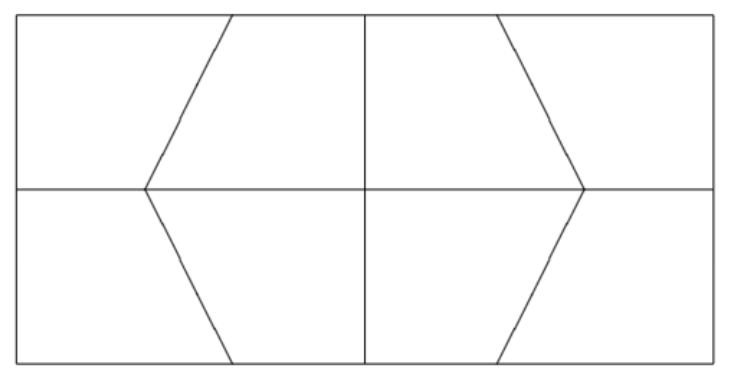
\includegraphics[scale=0.3]{images/ex1.png}
    \caption{Множество искомых точек}
    \label{fig:ex1}
\end{figure}

\begin{definition}
    Пусть $A, B \in \mathcal{F},$ тогда $A, B$ называют \textit{совместными}, если $A \cap B \neq \varnothing$.
\end{definition}

\begin{example}
При подбрасывании игрального кубика:
\begin{itemize}
    \item Событие $A$: ``выпало четное число'' $\{2, 4, 6\}$;
    \item Событие $B$: ``выпало число, меньшее 3'' $\{1, 2\}$;
\end{itemize}
Они совместные, так как $A \cap B = \{2\}$ (исход ``2'' благоприятствует обоим событиям).
\end{example}

\begin{definition}
    \textit{Условная вероятность} события $A$ при условии наступления события $B$ определяется формулой: $$\mathbb{P}\left( A \mid B \right) = \frac{\mathbb{P}\left( A \cap B \right)}{\mathbb{P}\left( B \right)}, \qquad \text{если } \mathbb{P}\left(B\right) \neq 0.$$
\end{definition}

\section{Лекция 09.09.25}

hello

\end{document}